\documentclass[conference]{IEEEtran}
\usepackage{float}
% *** CITATION PACKAGES ***
%
%\usepackage{cite}
% cite.sty was written by Donald Arseneau
% V1.6 and later of IEEEtran pre-defines the format of the cite.sty package
% \cite{} output to follow that of the IEEE. Loading the cite package will
% result in citation numbers being automatically sorted and properly
% "compressed/ranged". e.g., [1], [9], [2], [7], [5], [6] without using
% cite.sty will become [1], [2], [5]--[7], [9] using cite.sty. cite.sty's
% \cite will automatically add leading space, if needed. Use cite.sty's
% noadjust option (cite.sty V3.8 and later) if you want to turn this off
% such as if a citation ever needs to be enclosed in parenthesis.
% cite.sty is already installed on most LaTeX systems. Be sure and use
% version 5.0 (2009-03-20) and later if using hyperref.sty.
% The latest version can be obtained at:
% http://www.ctan.org/pkg/cite
% The documentation is contained in the cite.sty file itself.
\usepackage{hyperref}
\hypersetup{
    bookmarks=true,         % show bookmarks bar?
    unicode=false,          % non-Latin characters in Acrobat’s bookmarks
    pdftoolbar=true,        % show Acrobat’s toolbar?
    pdfmenubar=true,        % show Acrobat’s menu?
    pdffitwindow=false,     % window fit to page when opened
    pdfstartview={FitH},    % fits the width of the page to the window
    pdftitle={My title},    % title
    pdfauthor={Author},     % author
    pdfsubject={Subject},   % subject of the document
    pdfcreator={Creator},   % creator of the document
    pdfproducer={Producer}, % producer of the document
    pdfkeywords={keyword1, key2, key3}, % list of keywords
    pdfnewwindow=true,      % links in new PDF window
    colorlinks=true,       % false: boxed links; true: colored links
    linkcolor=blue,          % color of internal links (change box color with linkbordercolor)
    citecolor=blue,        % color of links to bibliography
    filecolor=blue,      % color of file links
    urlcolor=blue           % color of external links
}
% *** GRAPHICS RELATED PACKAGES ***
%
\ifCLASSINFOpdf
  \usepackage[pdftex]{graphicx}
  \graphicspath{{img/}}
  \DeclareGraphicsExtensions{.pdf,.jpeg,.png}
\else
  % or other class option (dvipsone, dvipdf, if not using dvips). graphicx
  % will default to the driver specified in the system graphics.cfg if no
  % driver is specified.
  % \usepackage[dvips]{graphicx}
  % declare the path(s) where your graphic files are
  % \graphicspath{{../eps/}}
  % and their extensions so you won't have to specify these with
  % every instance of \includegraphics
  % \DeclareGraphicsExtensions{.eps}
\fi
% graphicx was written by David Carlisle and Sebastian Rahtz. It is
% required if you want graphics, photos, etc. graphicx.sty is already
% installed on most LaTeX systems. The latest version and documentation
% can be obtained at:
% http://www.ctan.org/pkg/graphicx
% Another good source of documentation is "Using Imported Graphics in
% LaTeX2e" by Keith Reckdahl which can be found at:
% http://www.ctan.org/pkg/epslatex
%
% latex, and pdflatex in dvi mode, support graphics in encapsulated
% postscript (.eps) format. pdflatex in pdf mode supports graphics
% in .pdf, .jpeg, .png and .mps (metapost) formats. Users should ensure
% that all non-photo figures use a vector format (.eps, .pdf, .mps) and
% not a bitmapped formats (.jpeg, .png). The IEEE frowns on bitmapped formats
% which can result in "jaggedy"/blurry rendering of lines and letters as
% well as large increases in file sizes.
%
% You can find documentation about the pdfTeX application at:
% http://www.tug.org/applications/pdftex


% *** ALIGNMENT PACKAGES ***
%
%\usepackage{array}
% Frank Mittelbach's and David Carlisle's array.sty patches and improves
% the standard LaTeX2e array and tabular environments to provide better
% appearance and additional user controls. As the default LaTeX2e table
% generation code is lacking to the point of almost being broken with
% respect to the quality of the end results, all users are strongly
% advised to use an enhanced (at the very least that provided by array.sty)
% set of table tools. array.sty is already installed on most systems. The
% latest version and documentation can be obtained at:
% http://www.ctan.org/pkg/array

% correct bad hyphenation here
\hyphenation{op-tical net-works semi-conduc-tor}

\begin{document}
%
% paper title
% Titles are generally capitalized except for words such as a, an, and, as,
% at, but, by, for, in, nor, of, on, or, the, to and up, which are usually
% not capitalized unless they are the first or last word of the title.
% Linebreaks \\ can be used within to get better formatting as desired.
% Do not put math or special symbols in the title.
\title{Towards an Automated Categorization and Rating System of Airbnb Listings in New York City}


% author names and affiliations
% use a multiple column layout for up to three different
% affiliations
\author{\IEEEauthorblockN{Jonathan Pichot, Fernando Melchor, and Avikal Somvanshi}
\IEEEauthorblockA{Center for Urban Science + Progress\\
New York University\\
New York, NY\\
\href{https://github.com/fernandomelchor/Airbnb_Project}{GitHub}}
}

% conference papers do not typically use \thanks and this command
% is locked out in conference mode. If really needed, such as for
% the acknowledgment of grants, issue a \IEEEoverridecommandlockouts
% after \documentclass

% use for special paper notices
%\IEEEspecialpapernotice{(Invited Paper)}

% make the title area
\maketitle

% As a general rule, do not put math, special symbols or citations
% in the abstract
\begin{abstract}
Machine Learning techniques from all ranges of complexity are used to analyze datasets. Unsupervised classification could be used to enhanced our understanding of a system by analyzing the classification outcome. While humans are good at classifying things visually, when multi-dimensionality is involved, machine learning can help us to close this gap and enhance our understanding. This report applies an unsupervised classification technique to Airbnb listings in New York City with the purpose of developing an automated categorization and rating system for listings to be used by consumers and Airbnb itself.
\end{abstract}

\section{Introduction}
\IEEEPARstart
Airbnb is an online platform for residents of cities around the world to rent space in their homes and apartments.
Founded in 2008, Airbnb's mission is to help people "monetize their extra space." They've
been very successful, with over 3 million listings in over 65,000 cities worldwide.\cite{airbnb_about_us}
Since Airbnb listings are short-term housing provided by residents, the quality of the space
can vary drastically in quality, appointment, and amenities. The primary way Airbnb differentiates
its housing options is by the nature of the room. There are three options: shared, private, or entire home. A shared listing
is a shared space with the host, often on a couch in a living room. A private listing has
a door, usually a bedroom. And finally, a host can rent their entire home or apartment for a period of time.

Airbnb allows hosts to list the attributes of their listing, including photos, access to
technology, parking, washer/dryer, and other amenities. Past guests can leave reviews
that give further context to the quality of the place. But Airbnb does not rate the neighborhood
or location of the listing itself. For some more popular destinations, Airbnb does provide
neighborhood guides on their website.

This project will explore the possibility of creating a machine-learning driven
categorization system of Airbnb listings in New York City. A rating system similar to
those a guidebook might provide, giving a tourist an idea of what kind of amenities are found
around the listing. This project will focus on a combination of neighborhood attributes in the 
vicinity of the listing and some attributes on the listing itself.

The classification system developed could be useful to tourists and Airbnb alike.
Using the system, Airbnb customers in New York City would get a better idea of the amenities available
in the neighborhood around their rental, and Airbnb could use the analysis to better understand
their listing inventory and customer preferences. Is there stronger demand for cheaper listings?
For listings with better public transit connectivity? For listings close to certain
kinds of amenities? There are several rich possible applications.

\section{Data and Methods}

\subsection{Airbnb Listings}
The Airbnb listings for New York City were collected from InsideAirbnb.com,\cite{insideairbnb} a
website run by a New York City-based housing activist named Murray Cox. The website
scrapes Airbnb's website for many cities around the world, creating snapshots of all
listings on the site in a city on a given day. The data used in this analysis was from the
scrape of New York City on March 2nd, 2017.

The scraped data includes a lot of relevant information that was used in the analysis
including the price of the listing, how many reviews have been posted on it, its
approximate location (Airbnb does not publish the exact location of listings for security
reasons), the minimum number of nights per booking, the room type (shared, private, entire), and
many more.

\subsection{Outliers}
To make sure the analysis was performed on Airbnb listings that are actually being rented we
removed certain outliers. This left us with the listings with the below attributes:

\begin{itemize}
  \item Minimum of 7 or less nights per booking
  \item Listing price of \$500 or less
  \item At least 1 review
\end{itemize}

We feel a listing requiring a booking of greater than 7 nights begins to be considered a sublet rather
than short-term housing similar to a hotel room. Some listing had absurdly high listing prices. \$500 a night
is the equivalent of a high end hotel. Finally, by requiring at least 1 review we removed
listings that had likely never been booked. After removing all outliers we end up with
28,970 listings.

\subsection{Custom Attributes}
In addition to the attributes collected by Inside Airbnb, we added four custom attributes to each listing.
We developed using publicly available data. They are:

\begin{itemize}
  \item Median Household Income
  \item Craft Beer Count
  \item Specialty Coffee Count
  \item Connectivity Score
\end{itemize}

\subsection{Median income}
Median income of an area is a good indicator of safety of the area apart from being a class marker. Higher income neighborhoods doesn't necessarily translate into better access to amenities like cafes, restaurants and public transit (for instance Upper East Side) which might be critical for a tourist-traveler visiting the city for short duration.

Median income information was sourced from American Community Survey of 2015. Information was collected at Census block group level and each Airbnb listing was assigned the median income score of the census block group they were located in.

\subsection{Craft Beer and Specialty Coffee Counts}
One way to distinguish a neighborhood is to identify the kinds of businesses it can support.
Certain kinds of businesses cater to certain tastes. Two kinds of establishments that have
become popular in what could be called the taste-making young professionals' class is
specialty coffee (also referred to as third-wave coffee) and craft beer. The density
of these kinds of establishments in a neighborhood should work as a good indicator of
the kind of clientele a certain neighborhood attracts.

The location of specialty coffee shops and breweries were collected using Yelp's API.\cite{yelp_api}
All coffeeshops in New York City that were returned from the API when searching for the
string 'third wave coffee' were collected. Similarly, all breweries that were returned
from the API when searching for 'brewery' were also collected. This resulted in lists of
375 coffeeshops and 67 breweries.

These lists were then run through Mapzen's Isochrone API.\cite{mapzen_isochrone} This endpoint takes a point
and returns a polygon that represents all the area one can travel to given a certain time
and using a certain mode. Every coffeeshop and brewery was then merged on a polygon that
represented the area one could access in 10 minutes while walking (also known as a walkshed).

Finally, using these walksheds, the total number of specialty coffeeshops and breweries within
a 10 minute walk was calculated for every Airbnb listing. These totals gave us what we called
our 'coffee count' and 'beer count'. The distributions of these attributes can be seen in
Figure \ref{fig_coffee_count} and Figure \ref{fig_beer_count} respectively.

\begin{figure}[H]
\centering
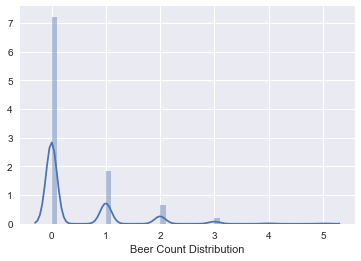
\includegraphics[width=3in]{beer_count}
\caption{Distribution of Beer Count}
\label{fig_beer_count}
\end{figure}

\begin{figure}[H]
\centering
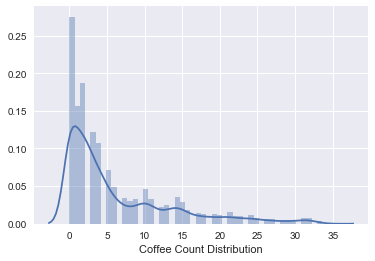
\includegraphics[width=3in]{coffee_count}
\caption{Distribution of Coffee Count}
\label{fig_coffee_count}
\end{figure}

\subsection{Connectivity Score}
We created a transportation connectivity score based on the listing's access to the subway system. The first task was the creation of a network representation of the NYC subway system by using the Metropolitan Transportation Authority (MTA) data that describes the service in each line. Links between the stations were created following the rules that the MTA uses to run the trains during weekdays at rush-hour. Figure \ref{Subway_Network} After the network of the subway system was complete, the average shortest path length was calculated for every station. In other words, from a single origin, the shortest path length to all the other possible station was calculated, then averaged and assigned to that station. The smaller the average shortest path length, the closest the station was to all the other stations in the system. Then, the value was reinterpreted to create score from 0 to 29, being 29 the closest station in the system.

To assign the score to the listings, the Mapzen's Isochrone API.\cite{mapzen_isochrone} was used again to create a 10 minute walking distance area from each station. The listings that fall inside the station's 10-minute walking distance generated area were assigned the station's connectivity score, if the listings fall within two or more stations ranges the score was added up.  Figure \ref{connect_score}

\begin{figure}[H]
\centering
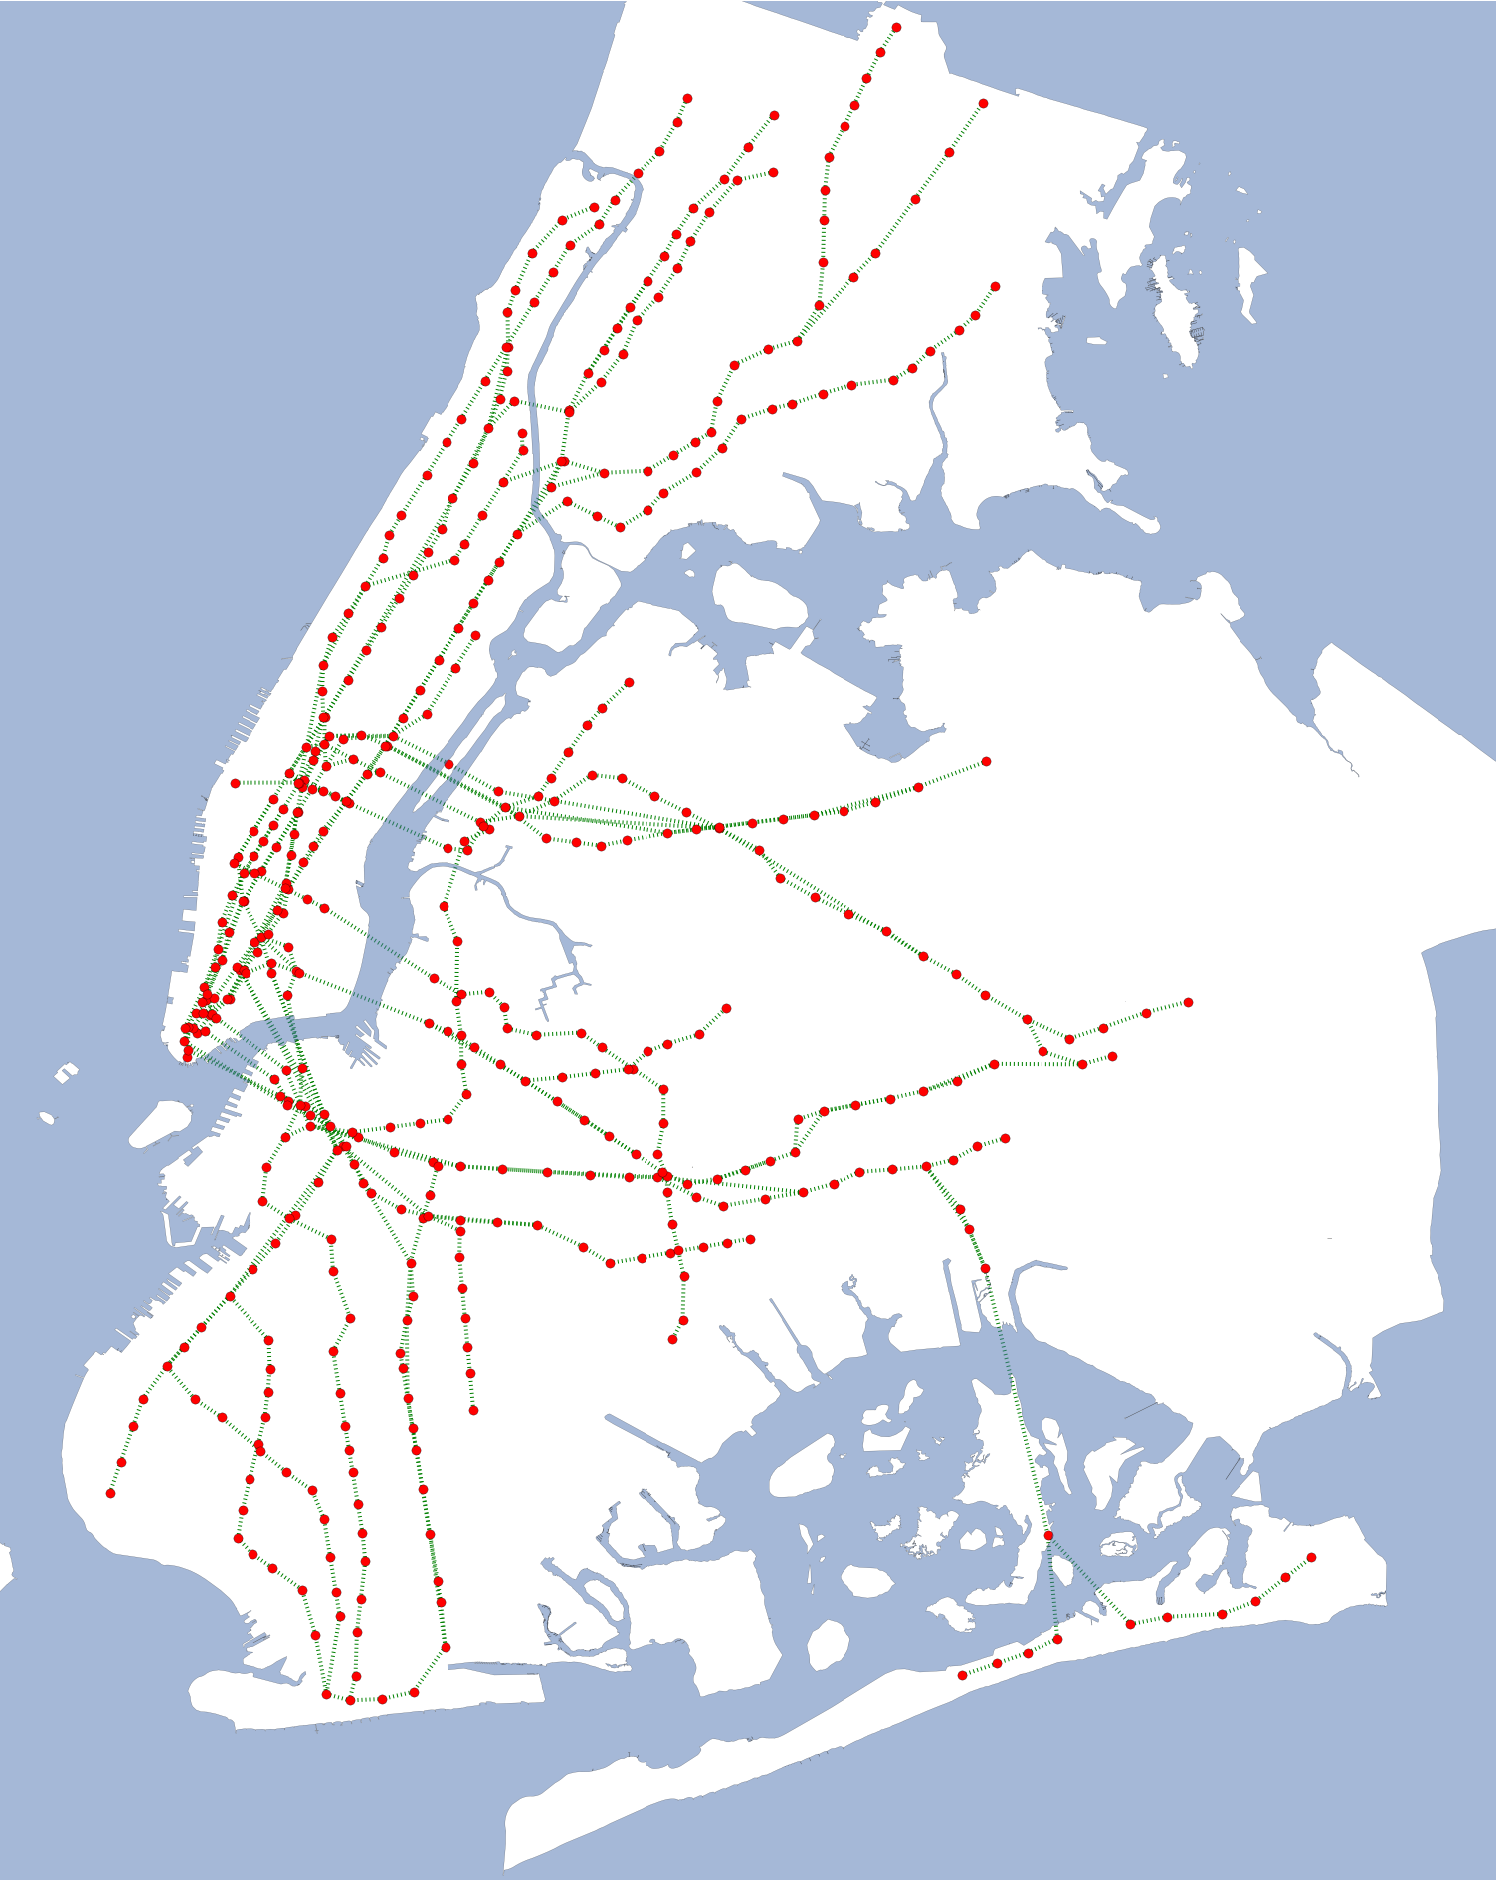
\includegraphics[width=3in]{Subway_Network}
\caption{Subway Network}
\label{Subway_Network}
\end{figure}


\begin{figure}[H]
\centering
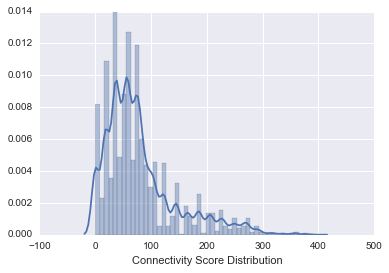
\includegraphics[width=3in]{connect_score}
\caption{Connectivity Score Distribution}
\label{connect_score}
\end{figure}

\section{Clustering}
To build an Airbnb listing classification model we ran KMeans clustering for 4 groups on our outlier-reduced listings
dataset. We clustered on 5 attributes:  Median Household Income, Craft Beer Count, Specialty Coffee Count, Connectivity Score,
and Listing Daily Price.

The size, in percentage of the total listings, of the clusters broke down as follows:

\begin{table}[h]
\caption{Percent breakdown of listings per KMeans classification}
\label{table:percent_listings}
\begin{center}
\begin{tabular}{l|l}
  Group & Percent of Listings\\
  \hline
  \hline
  0 & 55\\
  \hline
  1 & 2\\
  \hline
  2 & 12\\
  \hline
  3 & 31\\
\end{tabular}
\end{center}
\end{table}

\subsection{Listing Profiles}
Analyzing the four groupings given by our unsupervised clustering technique, we developed listing profiles of 
each as an example of how Airbnb might use a similar technique to have a better idea of the kinds of listings on their site
and to provide customers with an automated way to understand the neighborhood in which a listing is located. We gave our four
groupings unique names that captured their characteristics in a fun and memorable way. Our four groups are listed below along
with the color of their mapping in Table \ref{table:groupings}.

\begin{table}[h]
\caption{Groupings and average values of clustered attributes}
\label{table:groupings}
\begin{tabular}{l|l|l|l|l|l|l}
  Group Name & Color & Price & Income & Coffee & Beer & Conn.\\
  \hline
  \hline
  Normal People & blue & \$99 & \$25556 & 2.95 & 0.23 & 55.58\\
  \hline
  The 2\% & green & \$203 & \$183092 & 10.80 & 0.29 & 133.48\\
  \hline
  Central Action & red & \$184 & \$111362 & 11.74 & 0.38 & 134.60\\
  \hline
  Hip Kids & purple & \$153 & \$61687 & 9.86 & 0.73 & 98.10\\
\end{tabular}
\end{table}

\begin{figure}[h]
\centering
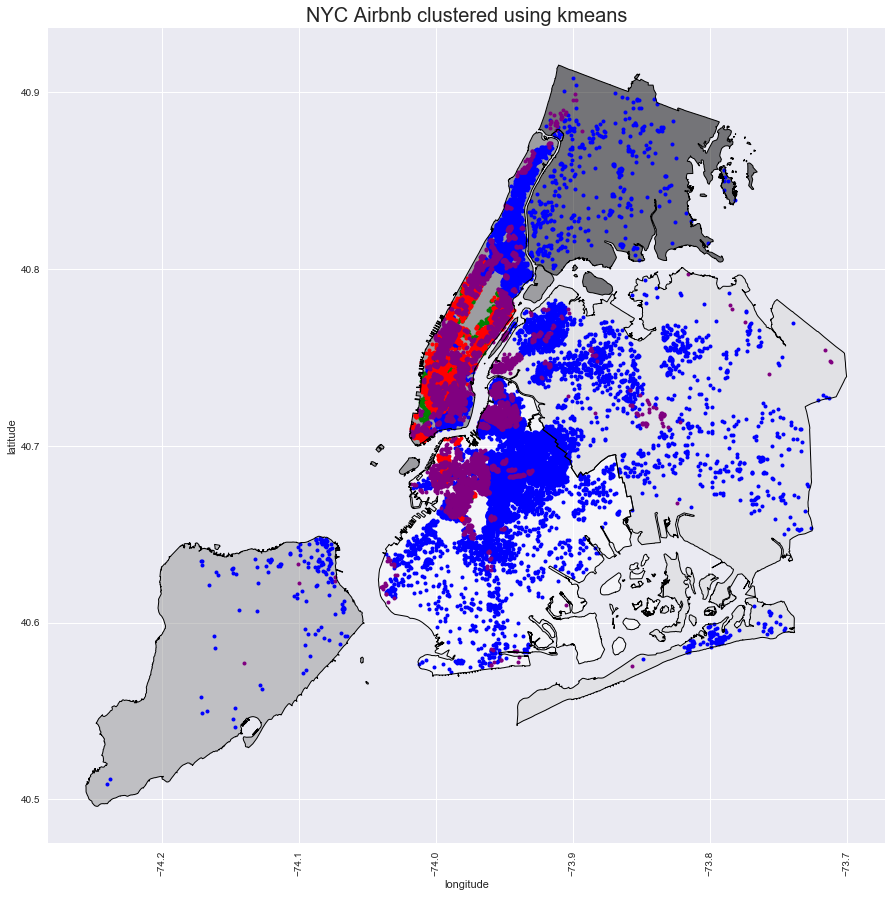
\includegraphics[width=3in]{all-clusters}
\caption{Map of Airbnb clusters}
\label{cluster-map}
\end{figure}

\subsubsection{Normal People}
The Normal People cluster represents 55\% of listings and has the lowest of all indicators, with a median income of \$25,556
and an average price of \$99 per night. It also has the lowest of our three custom indicators: coffee count, beer count, 
and connectivity score. As is clear on the map (Figure \ref{normal-map}), the Normal People are clustered outside of 
the more popular centers of Manhattan and Brooklyn (though Chinatown and the Lower East Side are still present). 
This is even more striking when looking at the density map of the Normal People (Figure \ref{ClusterNormalPeople}). As the map
reveals, the strongest cluster of Normal People are in Brooklyn in the adjoining neighborhoods to the hippest parts of the
borough.

\begin{figure}[h]
\centering
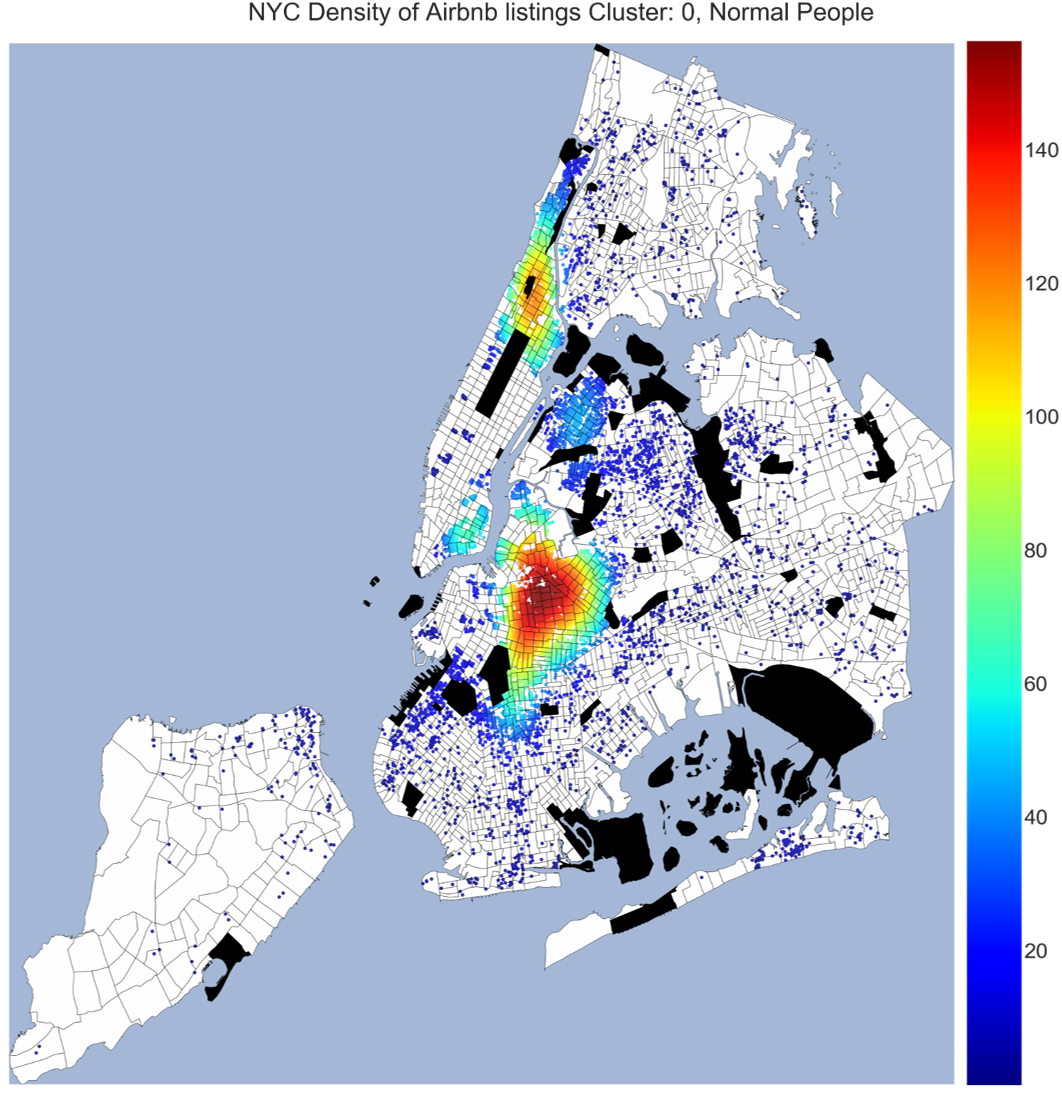
\includegraphics[width=3in]{ClusterNormalPeople}
\caption{Density graph of Normal People listings}
\label{ClusterNormalPeople}
\end{figure}

\begin{figure}[h]
\centering
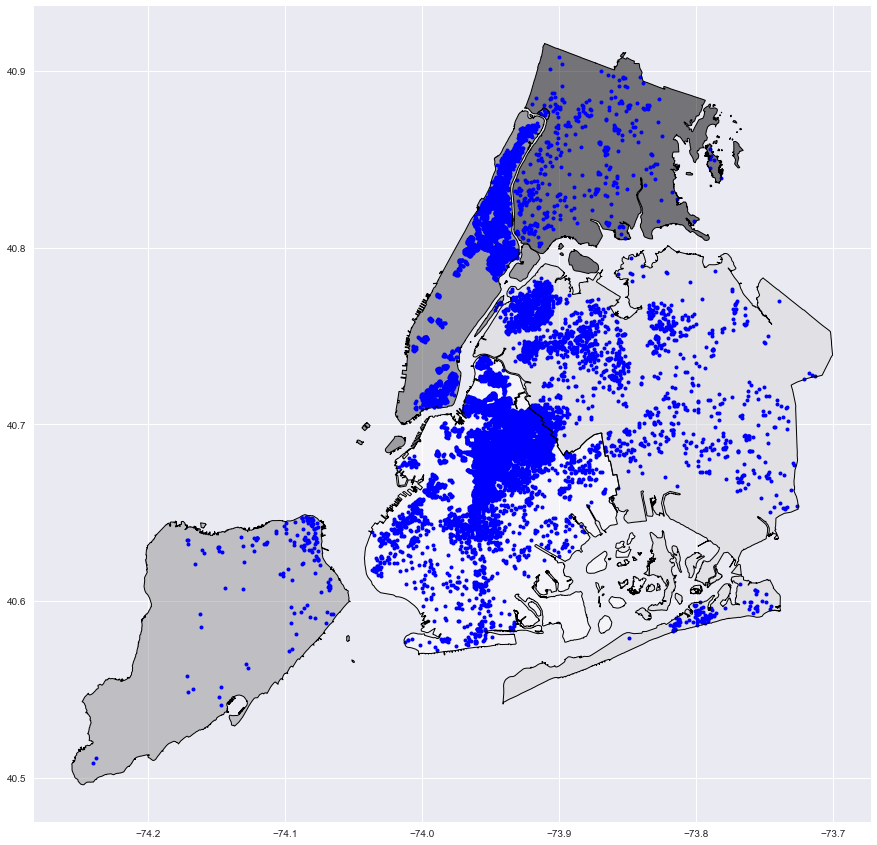
\includegraphics[width=3in]{group-1}
\caption{Map of Normal People listings}
\label{normal-map}
\end{figure}

\subsubsection{The 2\%}
The 2\%, as the name implies, represent only 2\% of the listings. These rarefied locations are also the most expensive with an
average price of \$203 a night. They are also clustered in the wealthiest neighborhoods with an average median income of around 
\$183,000. Interestingly, this high cost does not result in the highest scores in our custom indicators, with the 2\% having the
second highest coffee and connectivity scores and second to last beer score. The density map (Figure \ref{Cluster2percent}) of listings shows the highest
concentration of these listings in Midtown East (curiously, not far from Trump Tower).

\begin{figure}[h]
\centering
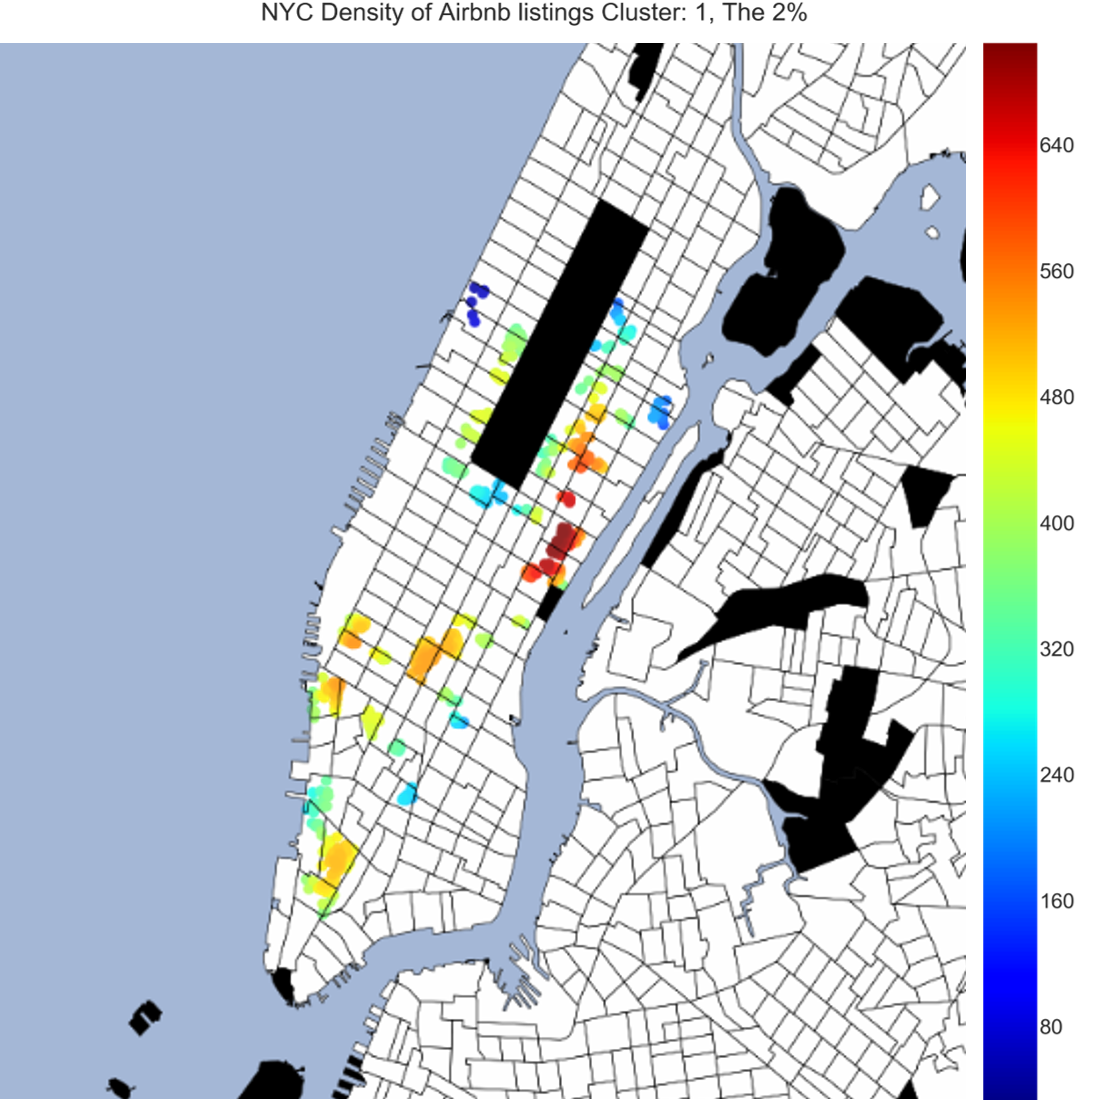
\includegraphics[width=3in]{Cluster2percent}
\caption{Cluster 1: The 2\%}
\label{Cluster2percent}
\end{figure}

\begin{figure}[h]
\centering
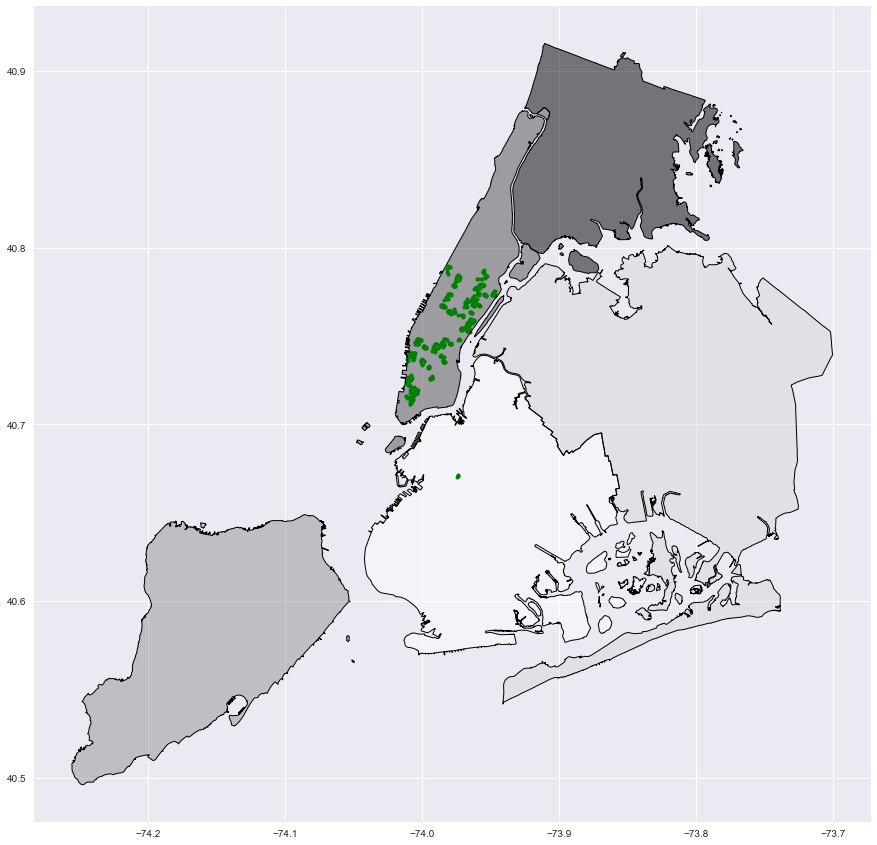
\includegraphics[width=3in]{group-2}
\caption{Map of the 2\% listings}
\label{2percent-map}
\end{figure}

\subsubsection{Central Action}
The Central Action grouping, as the name implies, is very centrally located to the core of Manhattan and the known tourist attractions
of the city. This location no doubt contributes to the groupings high price and general wealth, with the second highest average
nightly price and median income at \$183 and about \$111,000, respectively. This central clustering also puts these listings
very close to coffee and connectivity, representing the highest coffee score and connectivity scores of the model. The density map in 
Figure \ref{Clustercentral} reveals a strong clustering in Soho and Chelsea.

\begin{figure}[h]
\centering
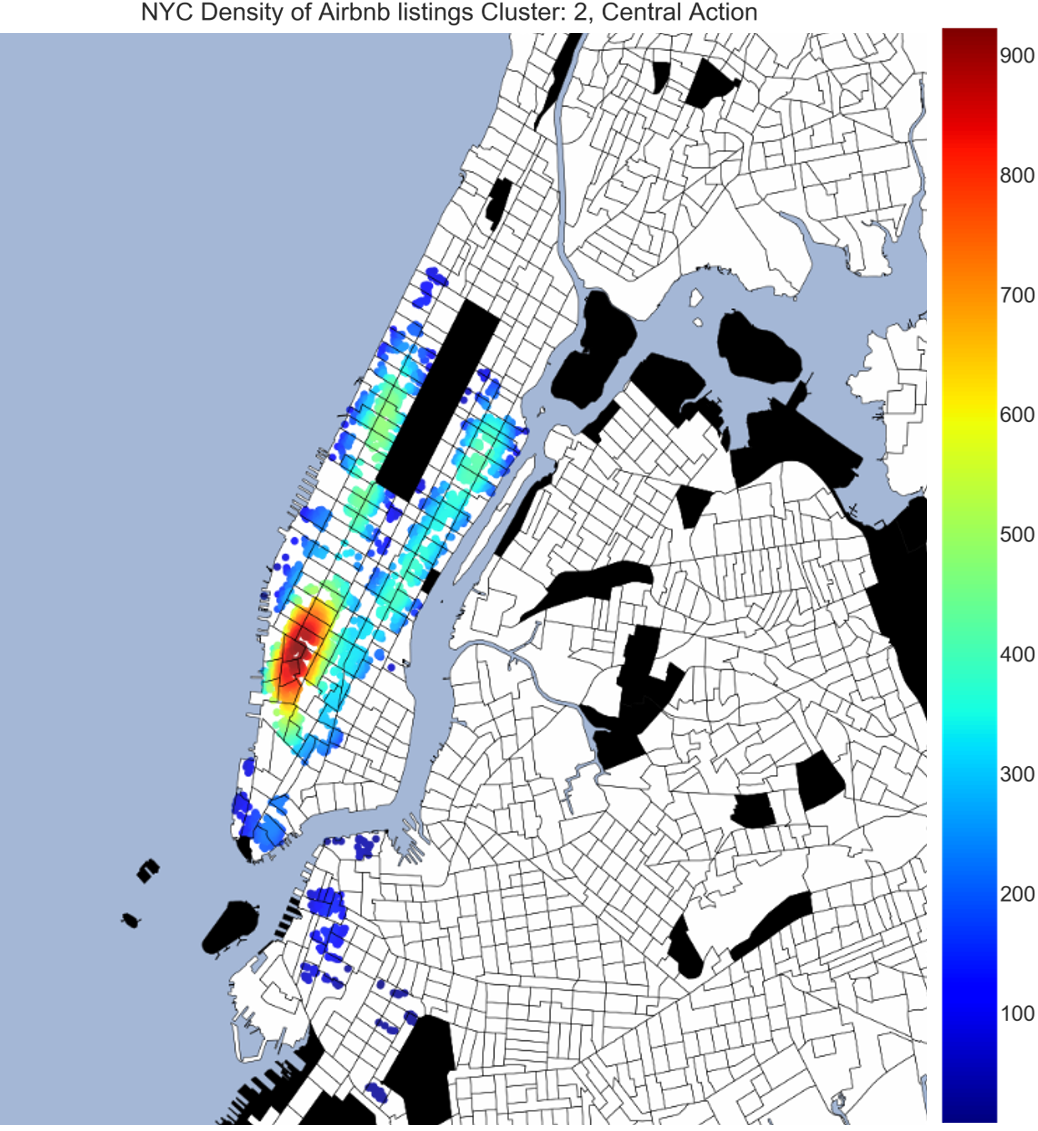
\includegraphics[width=3in]{Clustercentral}
\caption{Cluster 2: Central Action}
\label{Clustercentral}
\end{figure}

\begin{figure}[h]
\centering
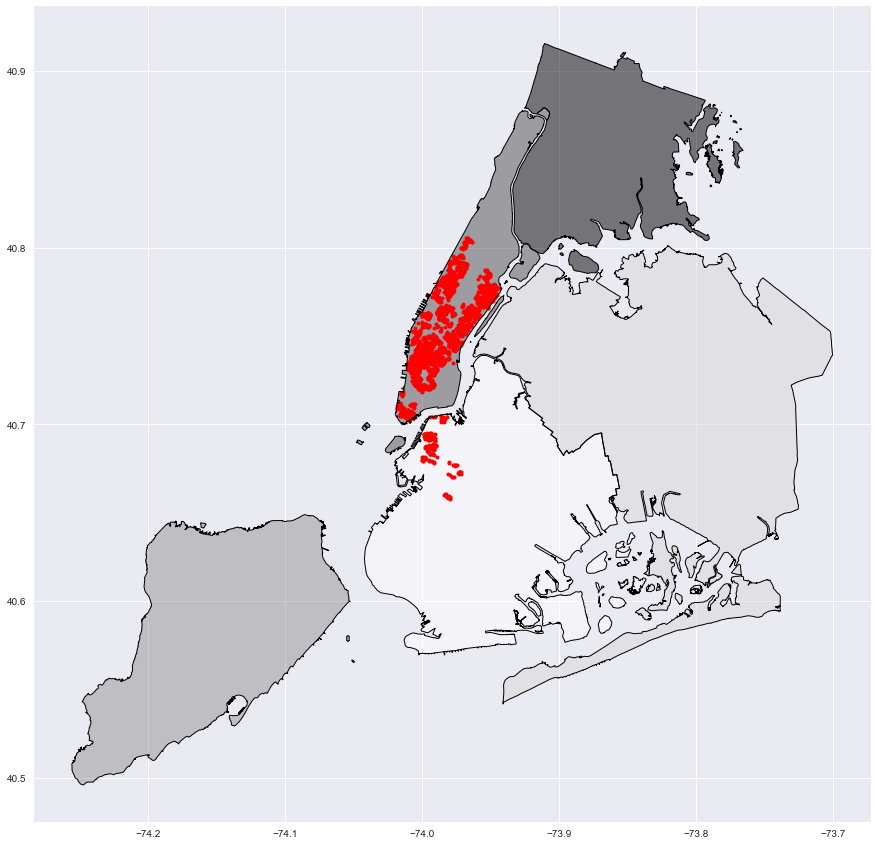
\includegraphics[width=3in]{group-3}
\caption{Map of Central Action listings}
\label{centralaction-map}
\end{figure}

\subsubsection{Hip Kids}
The Hip Kids, it appears, look for the cheapest tradeoff between accessibility, price, and amenities. Though this grouping has only
the third highest price and median income (at \$152 a night and about \$62,000 a year, respectively) it has the highest beer score
(by far) and a relatively high connectivity score and coffee score although it ranks third in both. As the density map reveals 
(Figure \ref{Clusterhip}), these listings are concentrated in the known hip centers of the Lower East Side and Williamsburg across
the East River. As such, there is likely a correlation between the lower density of areas like Williamsburg and the significantly
higher beer score, as breweries require space that is expensive to come buy in Manhattan.

\begin{figure}[h]
\centering
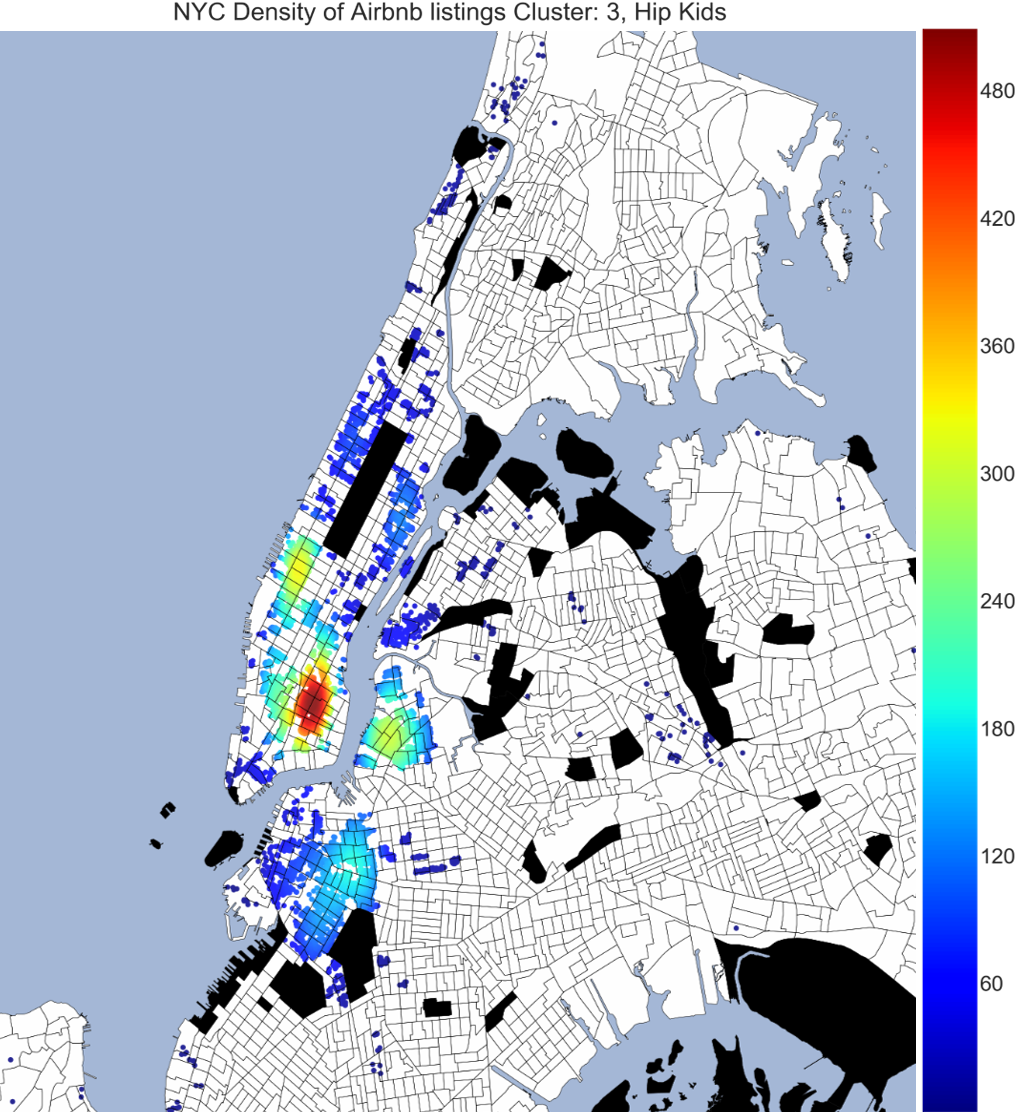
\includegraphics[width=3in]{Clusterhip}
\caption{Cluster 3: Hip Kids}
\label{Clusterhip}
\end{figure}

\begin{figure}[h]
\centering
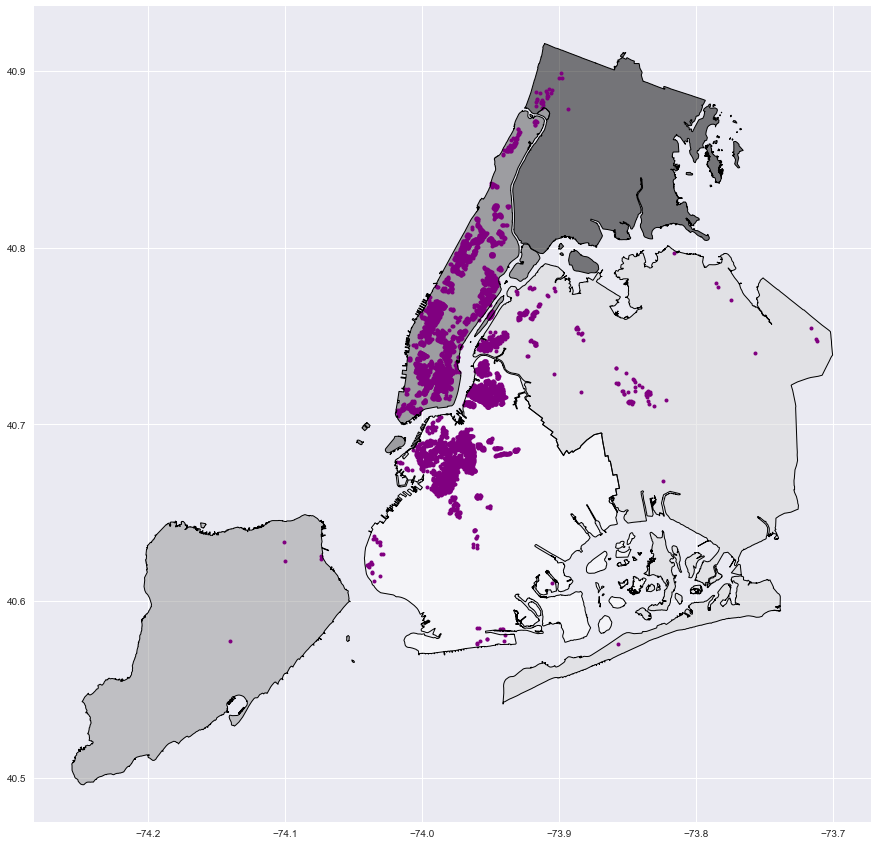
\includegraphics[width=3in]{group-4}
\caption{Map of Hip Kids listings}
\label{hipkids-map}
\end{figure}


\subsection{Validation}
The clustering results were cross validated using multiple semi-supervised classification techniques, namely Naive Bayes, Decision Trees, Bagging, Adaboosting, Gradient Boosting and Random Forest. The training data was defined such that these models could be used to predict the classes of new listings given nature of the neighborhood they are being offered in. 

Assessing the accuracy of the each of the semi-supervised learning model to predict the classes defined by K-means and Hierarchical clustering techniques helped understand the quality of the clusters/classes produced by the two methods(See Figure \ref{Validation Result table 1}). Each model was run 100 times and results reported in the tables are mean of all the 100 tests.

\begin{figure}
\centering
\caption{Validation results: Percent misclassified with all the features}
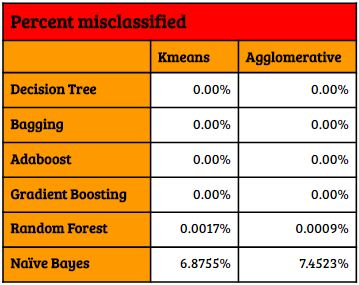
\includegraphics[width=3.5in]{ML_All_Features.JPG}
\label{Validation Result table 1}
\end{figure}

Another level of testing was carried out by dropping the most significant feature determining the initial clustering while carrying out cross-validation, to check how the performance of the select semi-supervised validation techniques gets affected (See Figure \ref{Validation Result table 2}). Degree of success in this test was expected to provide robustness of the whole methodology as in real life all the four features used in the model might not be available at all the time. Therefore, allowing the user to make a reasonably sound prediction by feeding only 75\% of the features to the model. 

\begin{figure}
\centering
\caption{Validation results: Percent misclassified without Median Income as a feature}
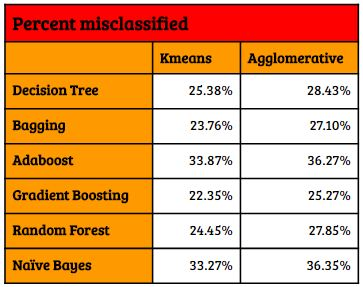
\includegraphics[width=3.5in]{ML_3_Features.JPG}
\label{Validation Result table 2}
\end{figure}

Results: Five out of six validation models yielded 100\% accuracy in predicting the class of new listing based on both K-Means and Hierarchical clustering. Naive Bayes model misclassified 6.8755\% of test data for K-Means and 7.4523\% of Hierarchical clustering. In the second round of validation, median income was dropped as one of the input features and accuracy of cross-validation models was found to be 66-78\% for K-Means and 62-74\% for Hierarchical clustering. Naive Bayes model was the worst performer for both clustering techniques while Random Forest with Gradient Boosting was the best but computationally the most taxing. 

\section{Discussion and Conclusion}
An automated classification of Airbnb listings is highly dependent on geography. As our groupings above demonstrate, most of our
attributes are highly determinate on geography. The location of coffee, beer, and transportation as well as price and median income
depends on where a listing is located. It is very difficult, when dealing with urban data sets, to extract features from a geographic
correlation. As such, any categorization of Airbnb listings will be highly dependent on the neighborhood it finds itself in. The 
model could be improved–for example, to take in to account attributes that would relate to child-friendly listings–by including
other attributes such as the size of the space, neighborhood factors that impact sound levels, etc. Geography is everything, it 
appears,in the emerging 'urban science' of applied data analysis on urban data sets.

The unsupervised clustering performed for this report is just an example of the kinds of applications possible with Airbnb listing
data. The Airbnb listings dataset is rich with attributes that could be used to create models for different purposes. One 
politically relevant use case, for which Inside Airbnb data has already been used several times, is to get a sense of the scale 
and strength of Airbnb listings on the cost of housing in New York City. Since this data does not include certain important attributes
to model the exact economic impact of a given listing, like the exact occupancy rate, a machine learning model could lend better
insight into how often a listing is rented given other attributes, like the number of reviews per month, the minimum length of stay, 
price, and other determinants on occupancy.


%
%\begin{figure*}[!t]
%\centering
%\subfloat[Case I]{\includegraphics[width=2.5in]{box}%
%\label{fig_first_case}}
%\hfil
%\subfloat[Case II]{\includegraphics[width=2.5in]{box}%
%\label{fig_second_case}}
%\caption{Simulation results for the network.}
%\label{fig_sim}
%\end{figure*}
%
% Note that often IEEE papers with subfigures do not employ subfigure
% captions (using the optional argument to \subfloat[]), but instead will
% reference/describe all of them (a), (b), etc., within the main caption.
% Be aware that for subfig.sty to generate the (a), (b), etc., subfigure
% labels, the optional argument to \subfloat must be present. If a
% subcaption is not desired, just leave its contents blank,
% e.g., \subfloat[].


% An example of a floating table. Note that, for IEEE style tables, the
% \caption command should come BEFORE the table and, given that table
% captions serve much like titles, are usually capitalized except for words
% such as a, an, and, as, at, but, by, for, in, nor, of, on, or, the, to
% and up, which are usually not capitalized unless they are the first or
% last word of the caption. Table text will default to \footnotesize as
% the IEEE normally uses this smaller font for tables.
% The \label must come after \caption as always.
%
%\begin{table}[!t]
%% increase table row spacing, adjust to taste
%\renewcommand{\arraystretch}{1.3}
% if using array.sty, it might be a good idea to tweak the value of
% \extrarowheight as needed to properly center the text within the cells
%\caption{An Example of a Table}
%\label{table_example}
%\centering
%% Some packages, such as MDW tools, offer better commands for making tables
%% than the plain LaTeX2e tabular which is used here.
%\begin{tabular}{|c||c|}
%\hline
%One & Two\\
%\hline
%Three & Four\\
%\hline
%\end{tabular}
%\end{table}

% trigger a \newpage just before the given reference
% number - used to balance the columns on the last page
% adjust value as needed - may need to be readjusted if
% the document is modified later
%\IEEEtriggeratref{8}
% The "triggered" command can be changed if desired:
%\IEEEtriggercmd{\enlargethispage{-5in}}

% references section

% can use a bibliography generated by BibTeX as a .bbl file
% BibTeX documentation can be easily obtained at:
% http://mirror.ctan.org/biblio/bibtex/contrib/doc/
% The IEEEtran BibTeX style support page is at:
% http://www.michaelshell.org/tex/ieeetran/bibtex/
% argument is your BibTeX string definitions and bibliography database(s)

\bibliographystyle{IEEEtran}
\bibliography{library}

% that's all folks
\end{document}
